\documentclass{elegantpaper}
\usepackage{datetime2}
\usepackage[T1]{fontenc}
\usepackage{graphicx}

\DTMusemodule{english}{en-GB}
\DTMnewdatestyle{short}{
  \renewcommand{\DTMdisplaydate}[4]{
    \DTMenglishmonthname{##2} \number##1\relax
  }
  \renewcommand{\DTMDisplaydate}{\DTMdisplaydate}
}
\newcommand{\shorttoday}{{\DTMsetdatestyle{short}\today}}
\renewcommand{\updatetext}{}

\graphicspath{{./images/}}
\DeclareEmphSequence{\bfseries,\itshape,\upshape}

\title{}
\author{Sin7Y, Applied R\&D Team\thanks{\url{https://twitter.com/Sin7Y_Labs}}}
\date{\shorttoday}

\begin{document}
    \maketitle
    \tableofcontents
    \section{add-biguint}
\label{add-biguint}

Take uint128 as example, the same as other texs.

\begin{enumerate}
    \item target
        implenment the addition of two biguints.
    \item constraints-logic
        \begin{itemize}
            \item equation for gate
            \item sumcheck between ouptput and limbs
            \item rangecheck for limbs
        \end{itemize}
    \item circuit layout
        \begin{figure}[!ht]
            \centering
            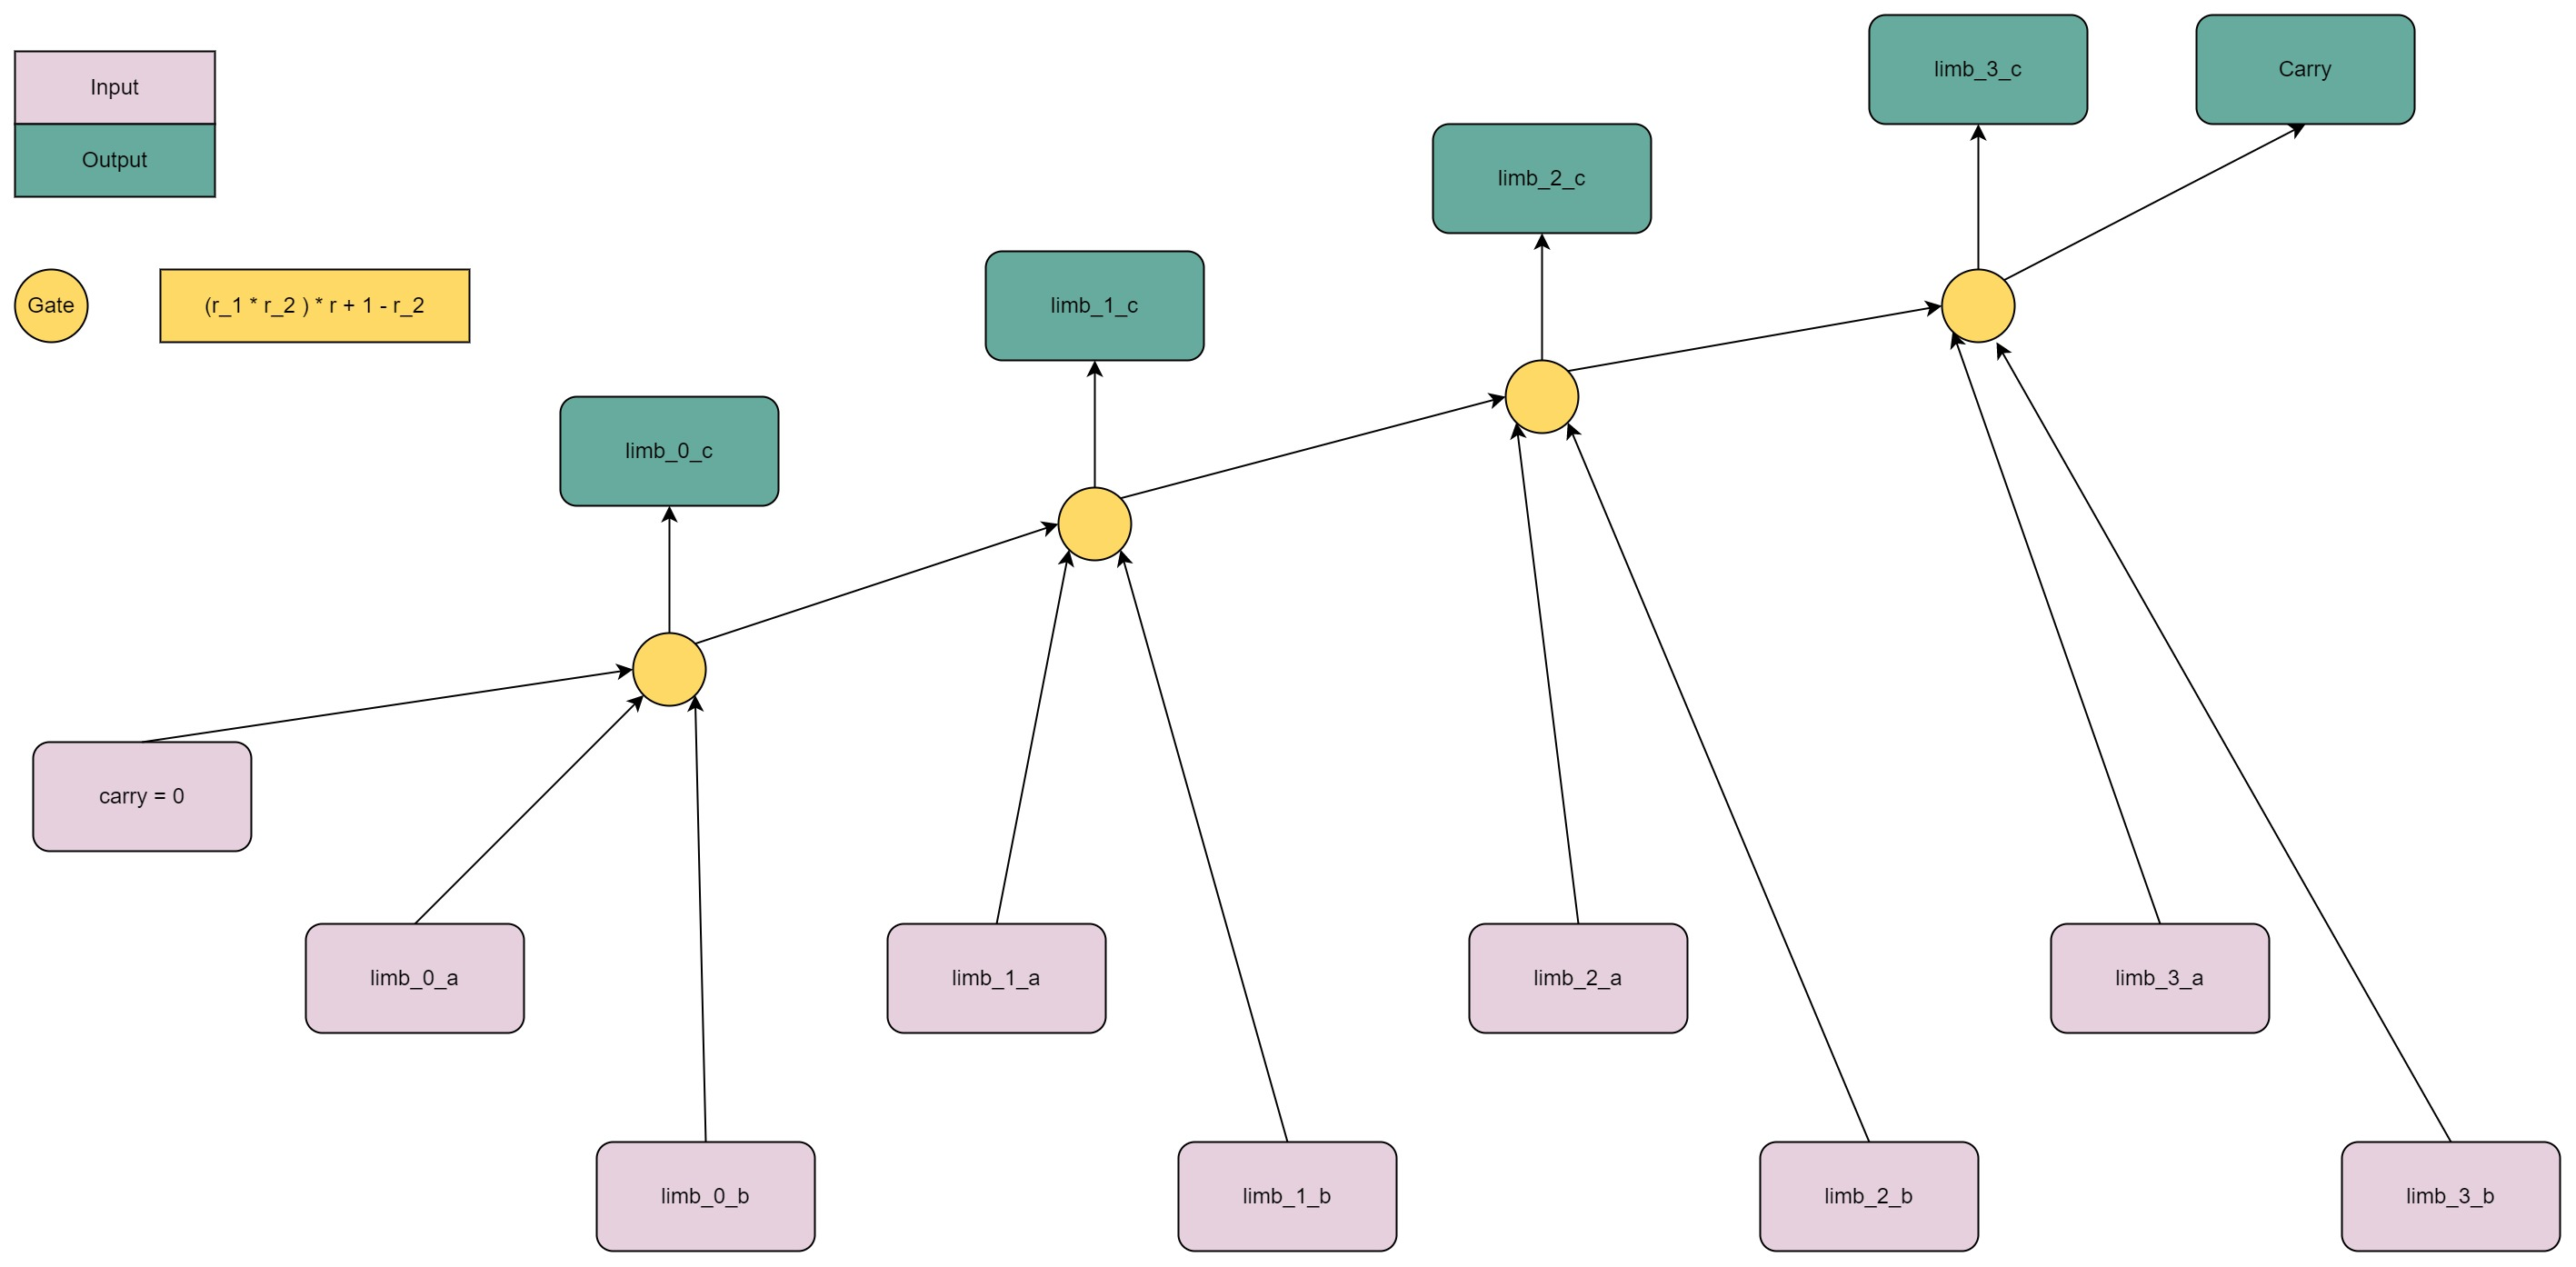
\includegraphics[width=0.8\textwidth]{add-biguint-circuit-layout.jpg}
            \caption{Add-biguint-circuit-layout}
            \label{fig:add-biguint-circuit-layout}
        \end{figure}

    \item trace layout
        \begin{figure}[!ht]
            \centering
            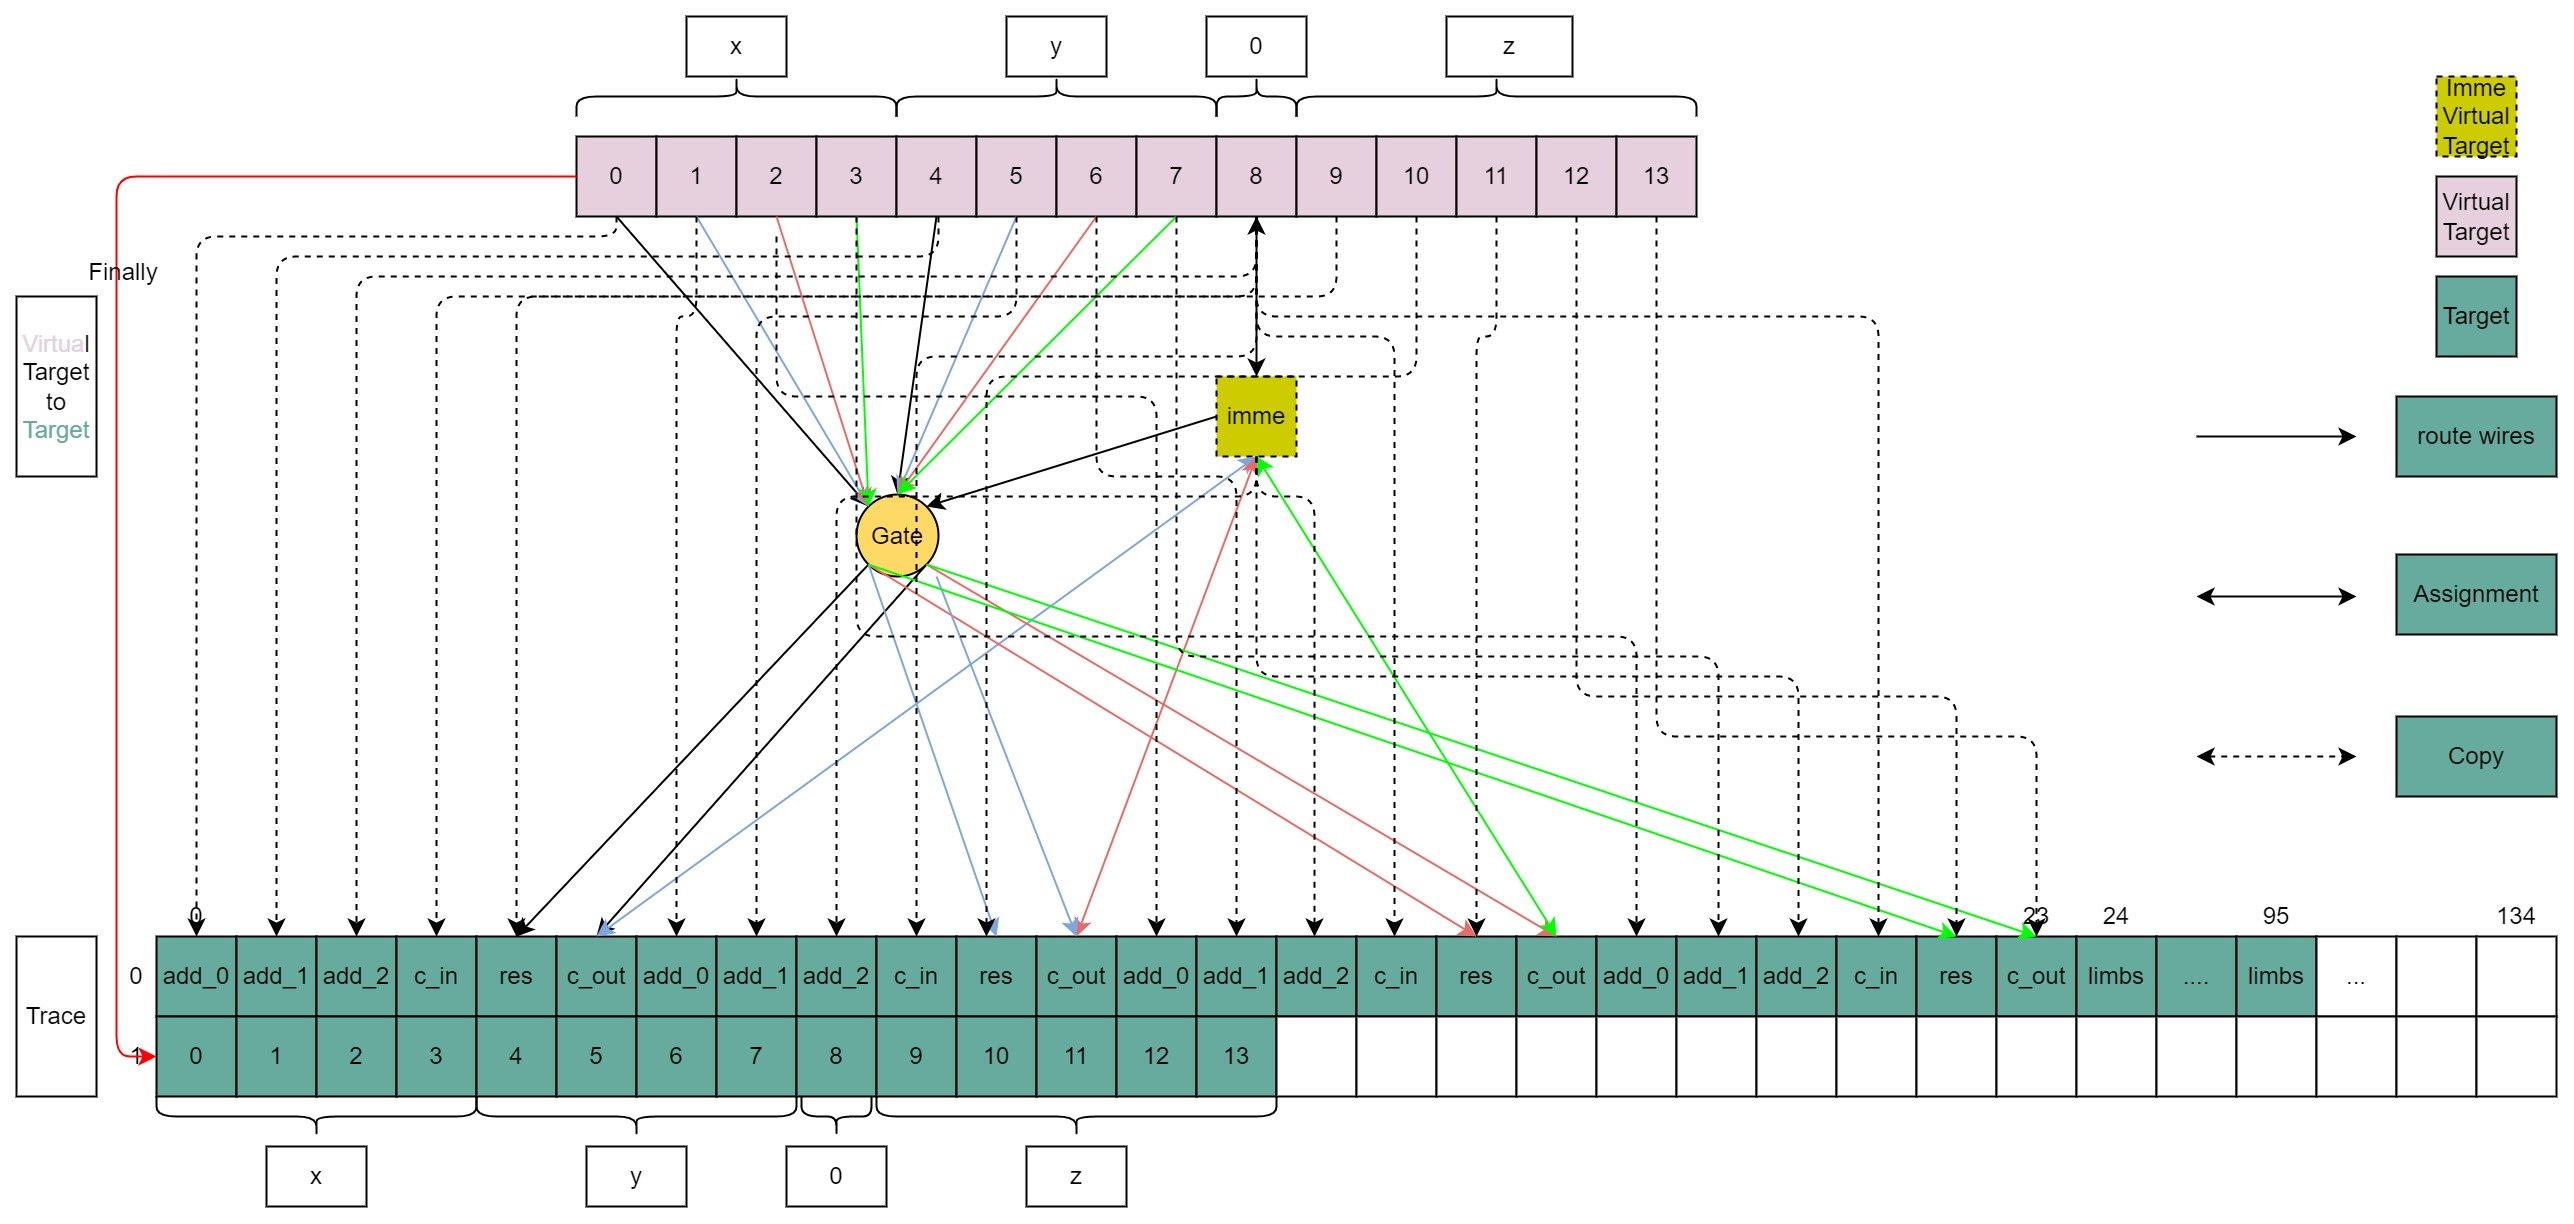
\includegraphics[width=0.8\textwidth]{add-biguint-trace-layout.jpg}
            \caption{Add-biguint trace layout}
            \label{fig:add-biguint-trace-layout}
        \end{figure}
    
    \item constraints-info and costs
        \begin{itemize}
            \item constraints-num: 5 * (3 + 32 / 2 + 4 / 2) = 105
            \item copy-constraints: 4 * 5 + 6 = 26
            \item max-degree: 4
            \item wires-num: 5 * (6 + 16 + 2) = 120
        \end{itemize}

    \item questions
        \begin{itemize}
            \item why not make rangecheck constraint for inputs?
            \item why not make copy constraint between cur-c-in and last-c-out?
        \end{itemize}

\end{enumerate}
    \section{sub-biguint}
\label{sub-biguint}

\begin{enumerate}
    \item target
        implenment the substraction of two biguints.
    \item constraints-logic
        \begin{itemize}
            \item equation for gate
            \item sumcheck for ouptput 
            \item rangecheck for limbs
        \end{itemize}
    \item circuit layout
        \begin{figure}[!ht]
            \centering
            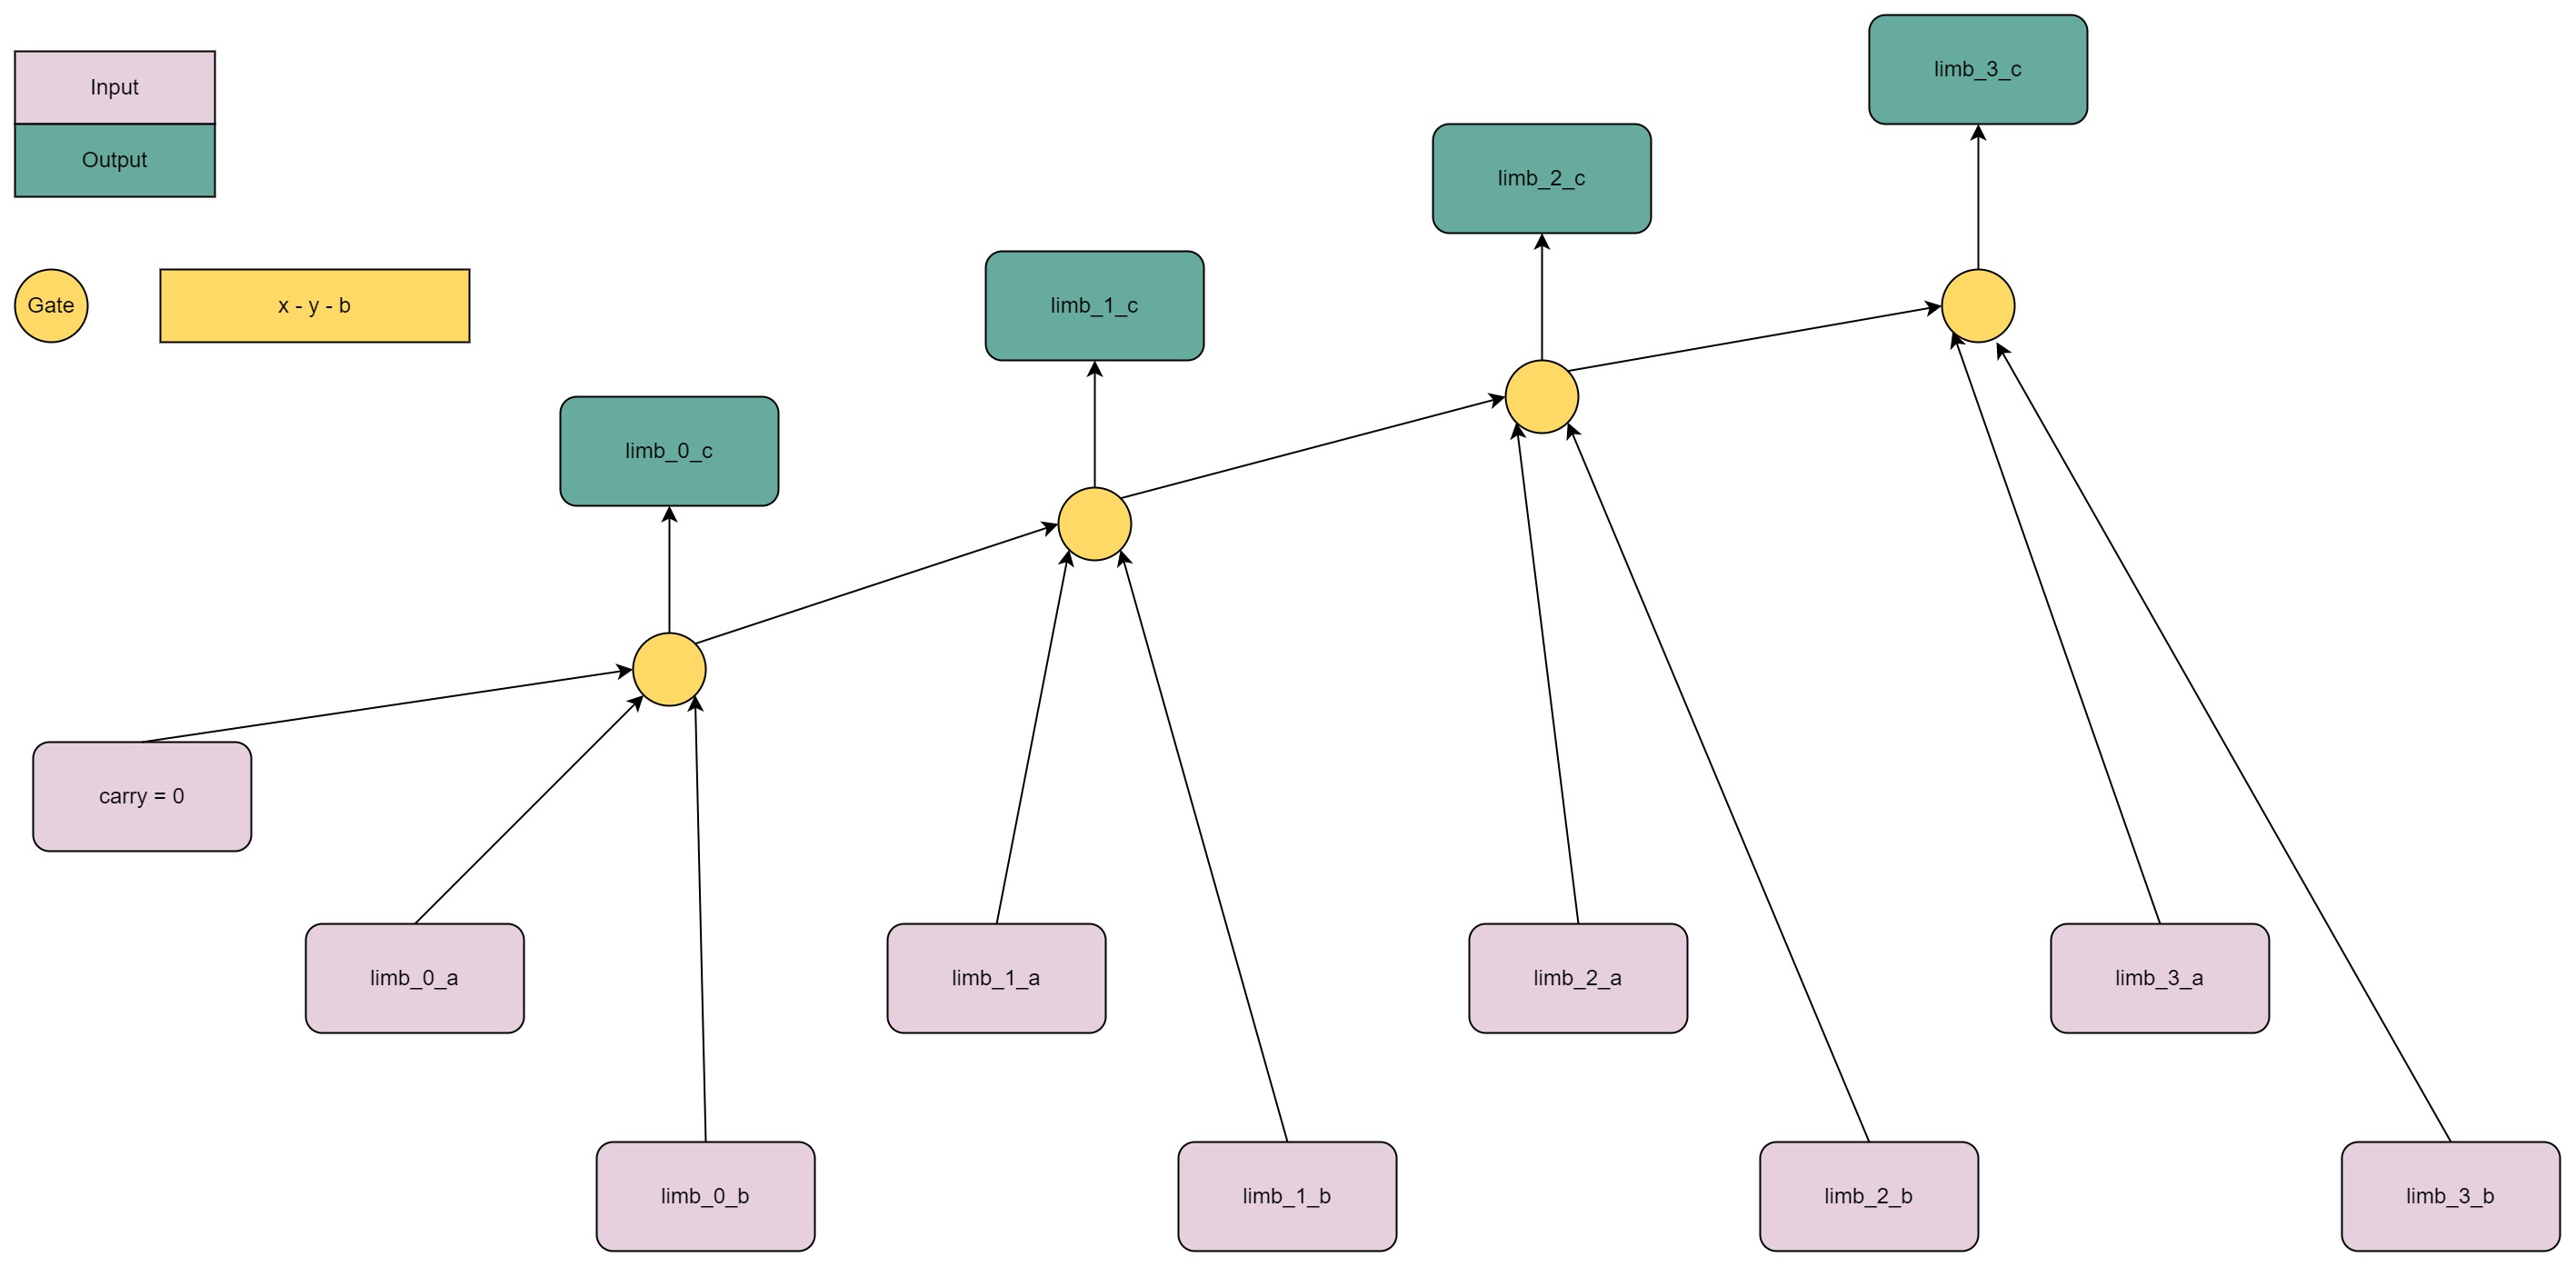
\includegraphics[width=0.8\textwidth]{sub-biguint-circuit-layout.jpg}
            \caption{Sub-biguint circuit layout}
            \label{fig:sub-biguint-circuit-layout}
        \end{figure}

    \item trace layout
        \begin{figure}[!ht]
            \centering
            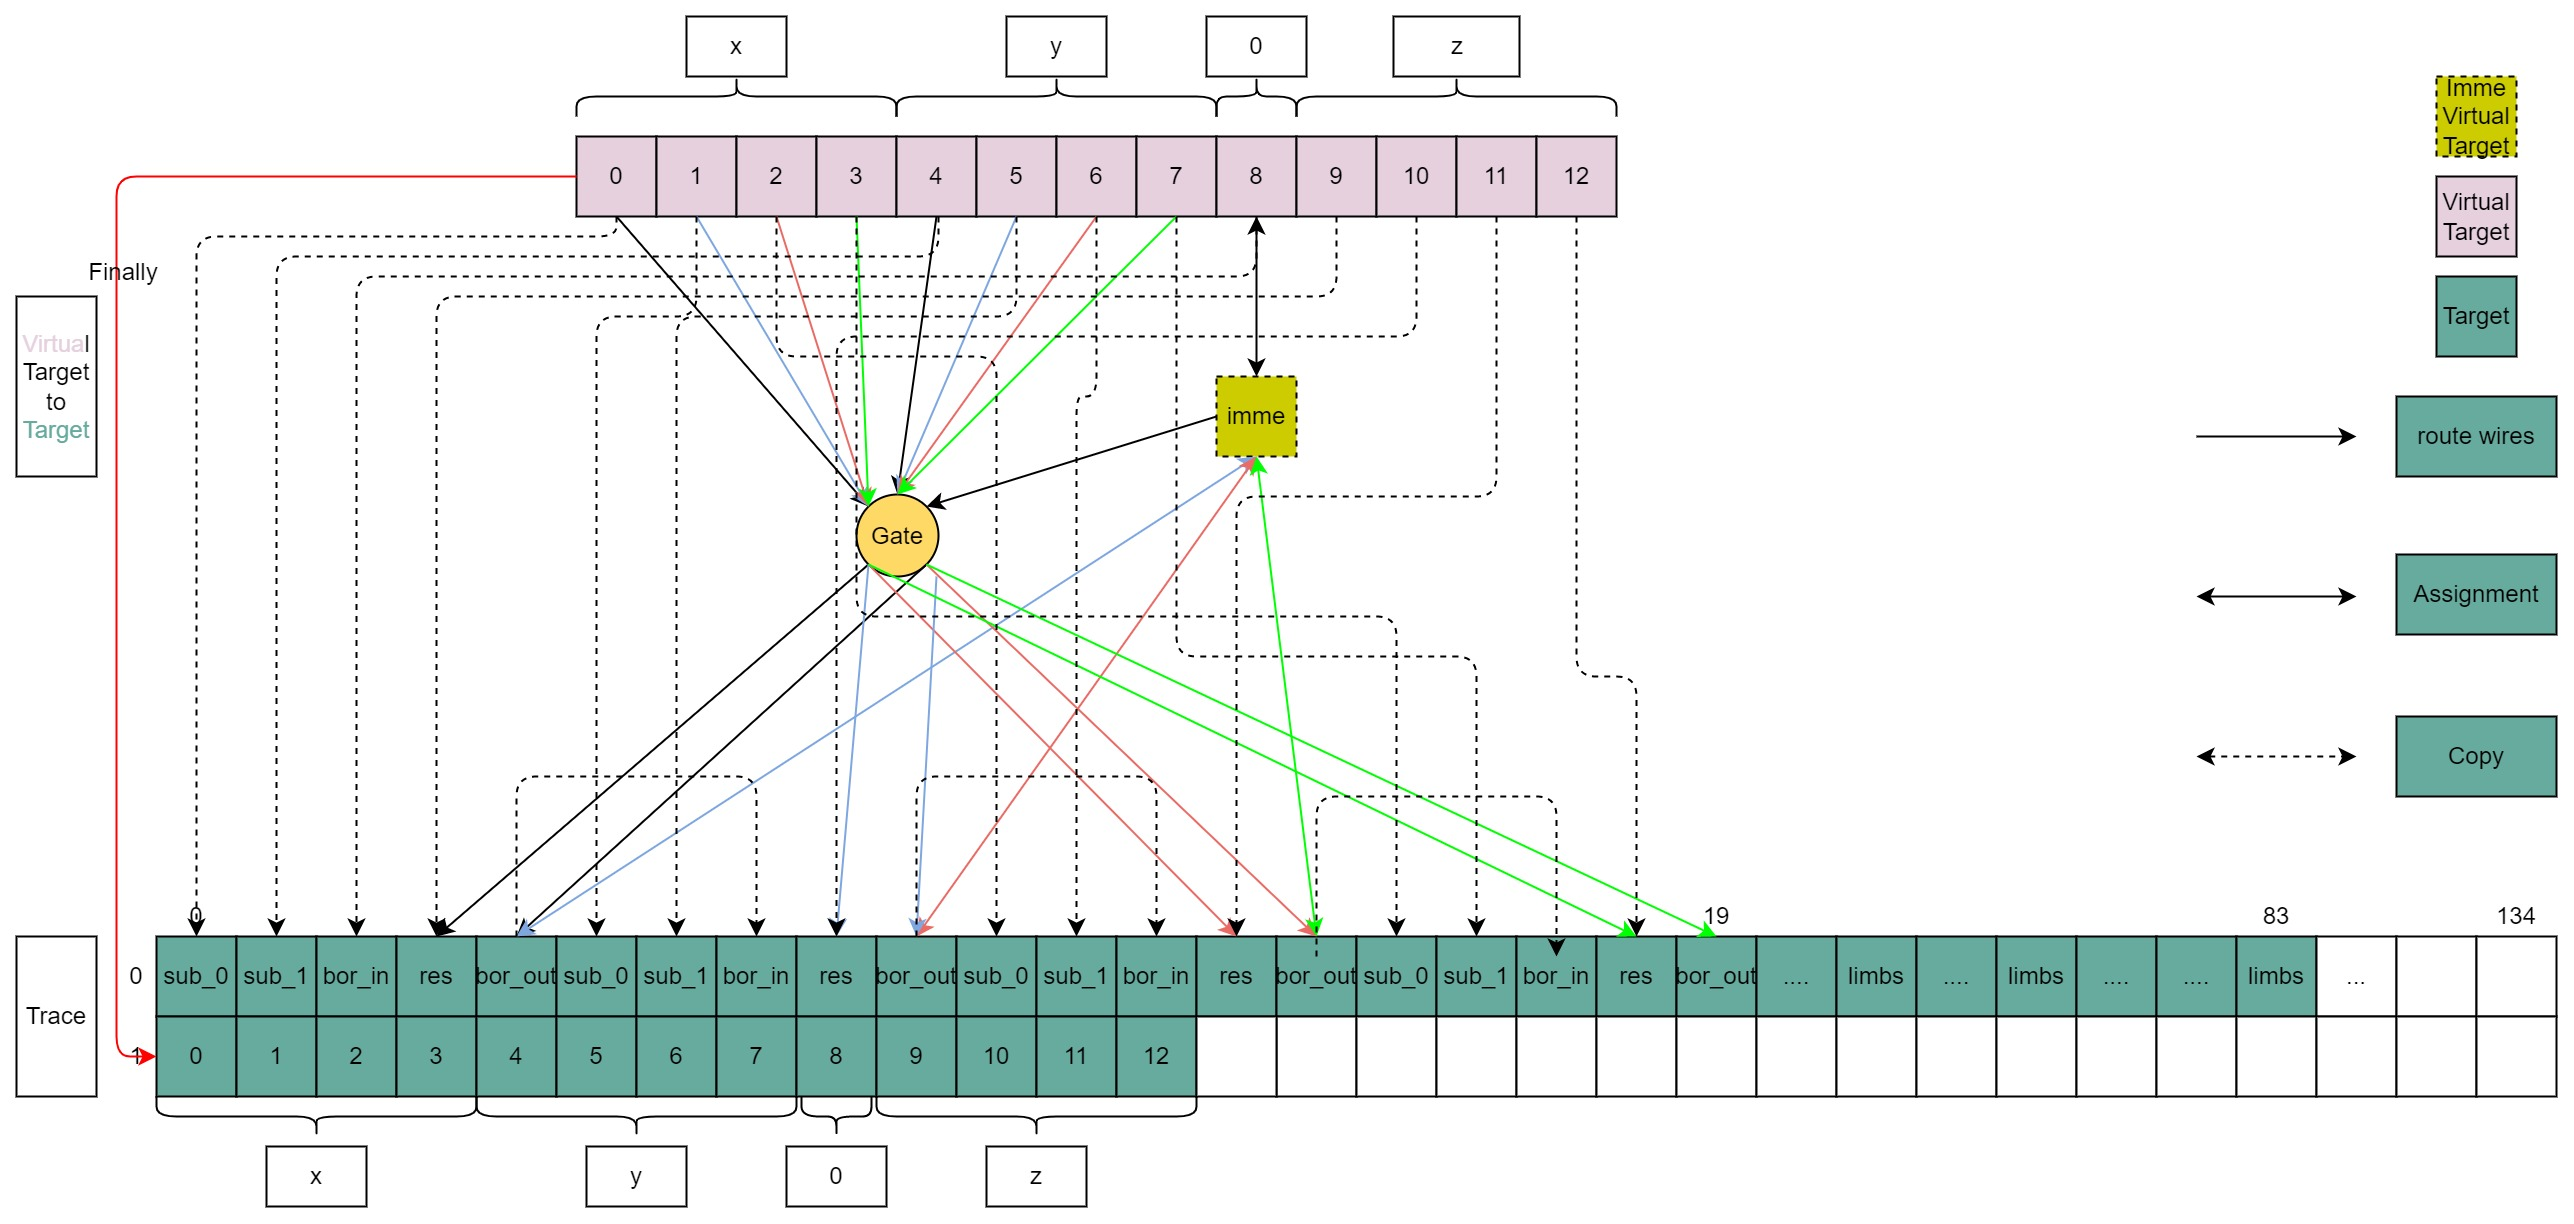
\includegraphics[width=0.8\textwidth]{sub-biguint-trace-layout.jpg}
            \caption{Sub-biguint trace layout}
            \label{fig:sub-biguint-trace-layout}
        \end{figure}
    
    \item constraints-info and costs
        \begin{itemize}
            \item constraints-num: 6 * (3 + 32 / 2) = 114
            \item copy-constraints: 16
            \item max-degree: 4
            \item wires-num: 6 * (5 + 16) = 126
        \end{itemize}

    \item questions
        \begin{itemize}
            \item why not make rangecheck constraint for inputs?
            \item Could try to use the same constraint with add-gate.
        \end{itemize}

\end{enumerate}
    \section{mul-biguint}
\label{mul-biguint}

\begin{enumerate}
    \item target
        \begin{itemize}
            \item implenment the multiplication of two biguints
        \end{itemize}
    \item constraints-logic
        \begin{itemize}
            \item equation for gate.
            \item sumcheck between ouptput and limbs
            \item rangecheck for limbs
        \end{itemize}
    \item mul-process layout
        \begin{figure}[!ht]
            \centering
            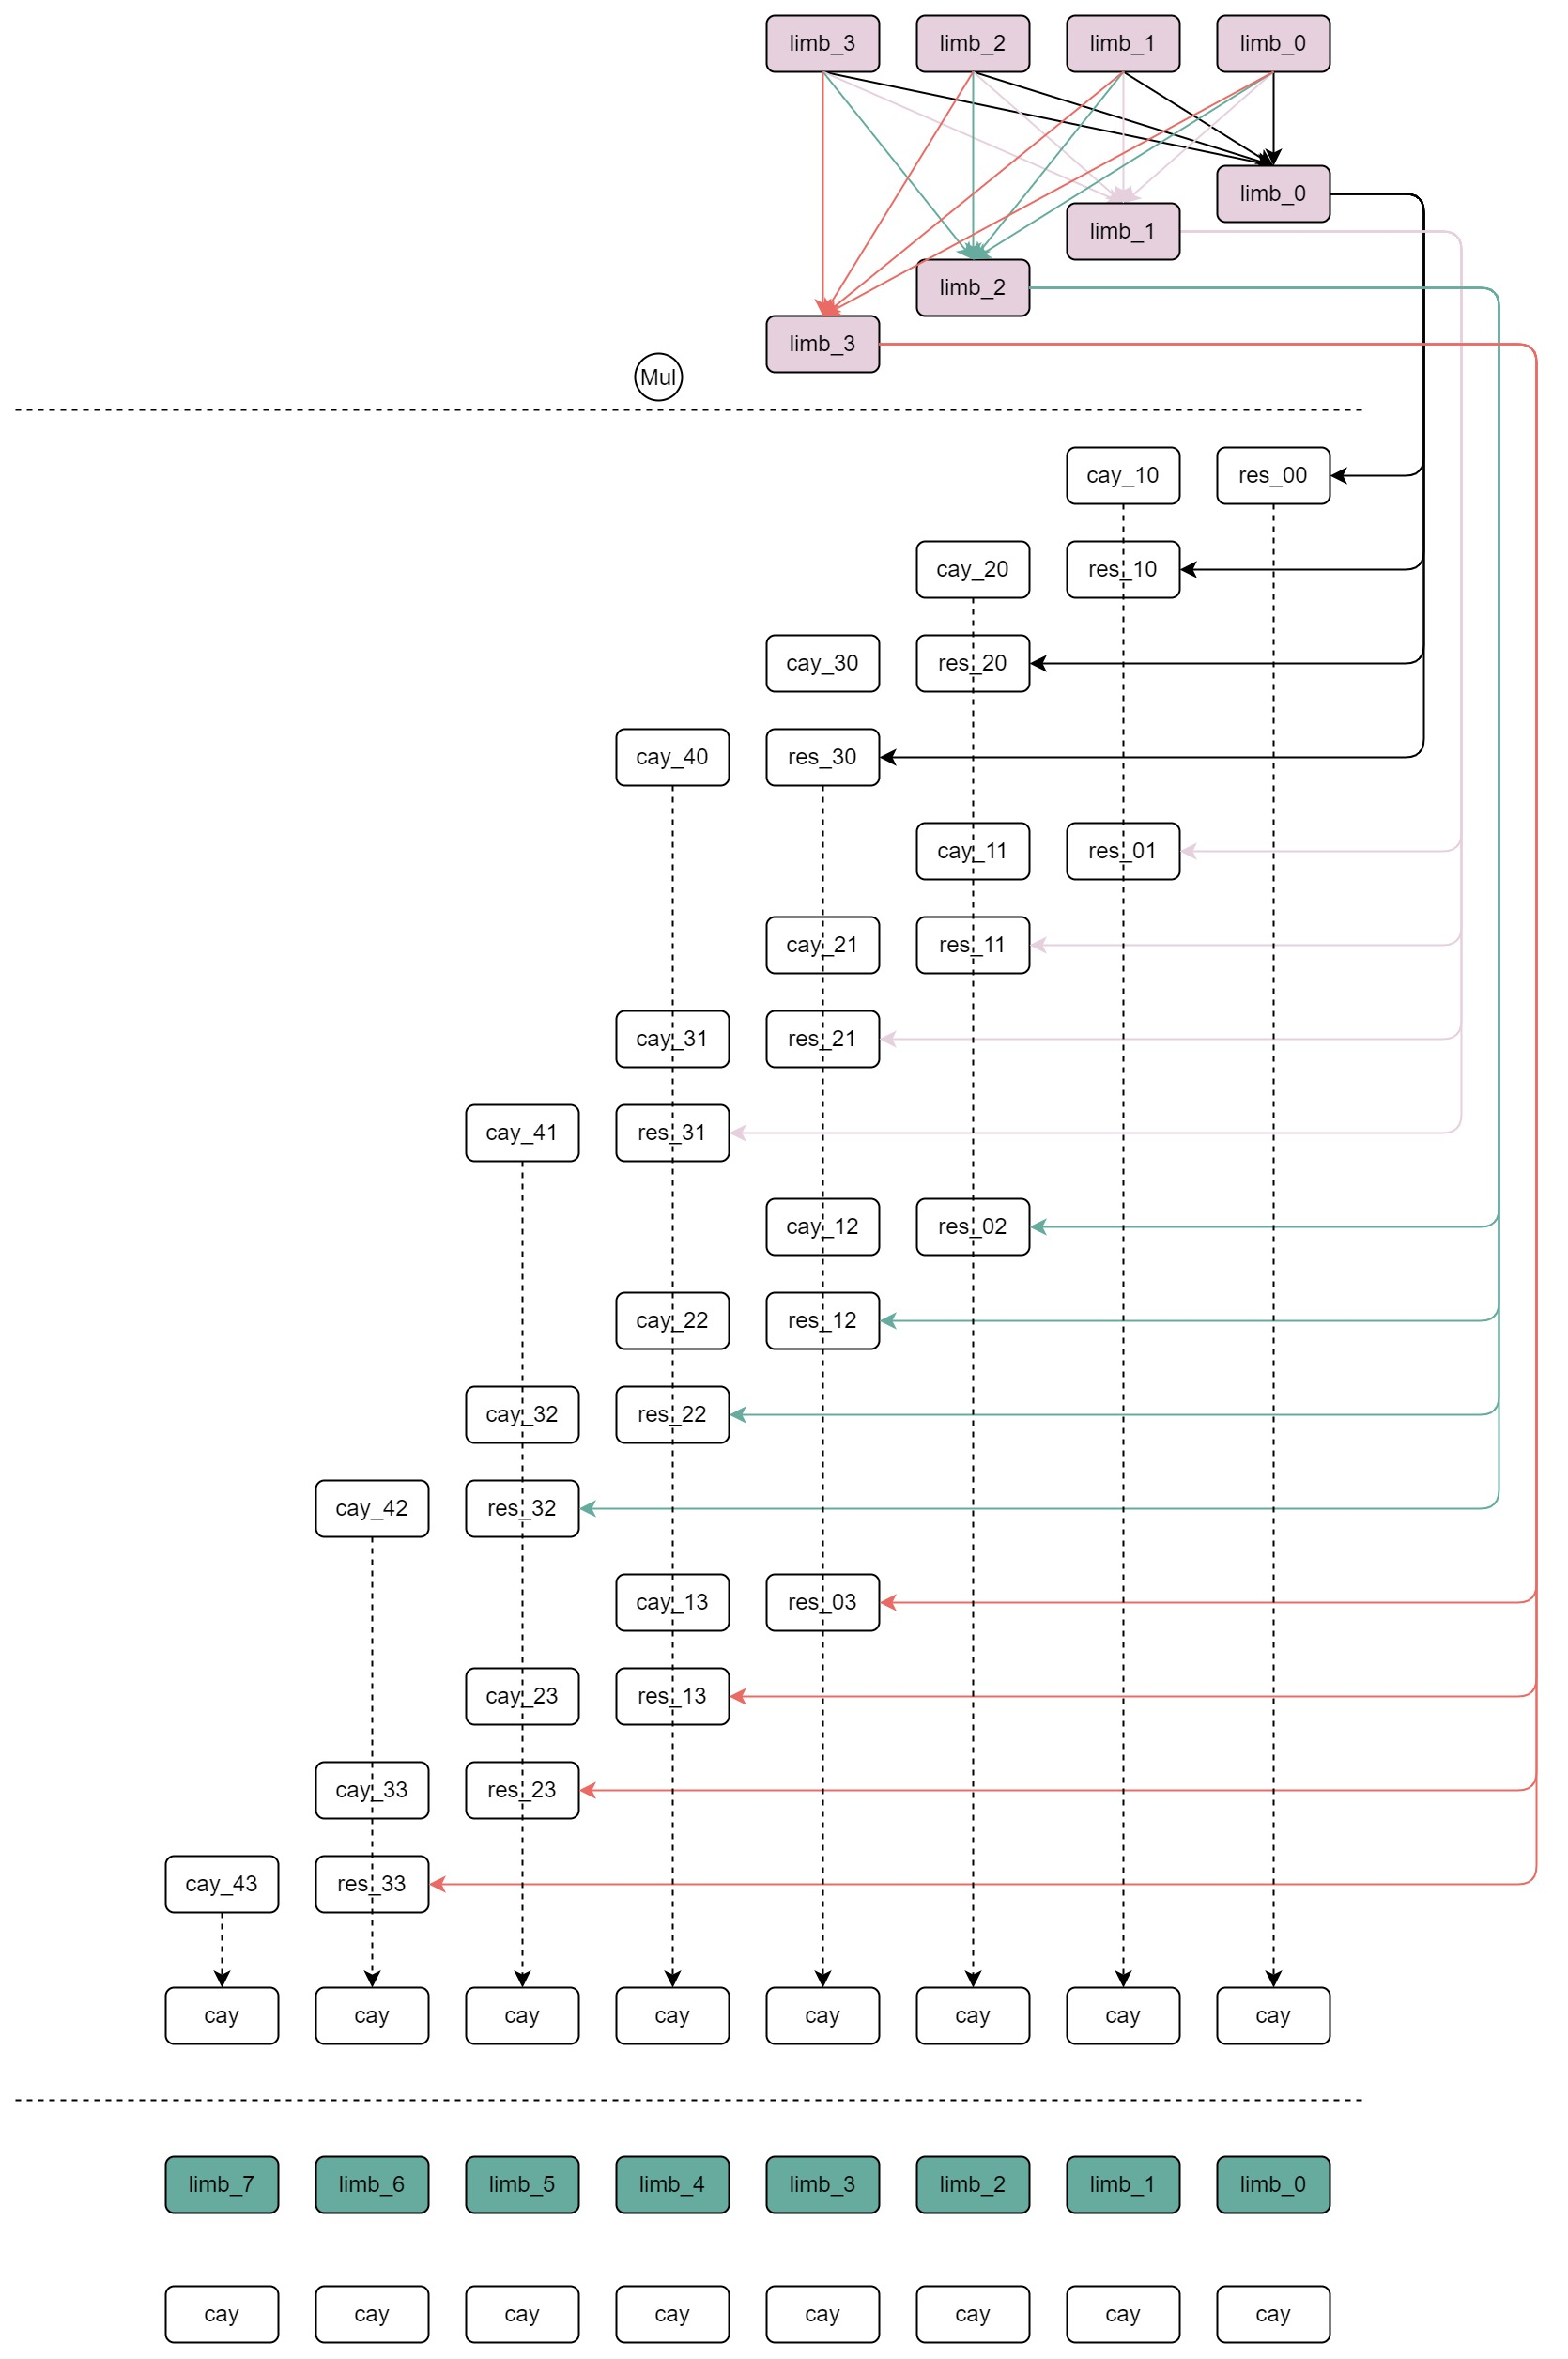
\includegraphics[width=0.8\textwidth]{mul-biguint-layout.jpg}
            \caption{Mul-biguint layout.jpg}
            \label{fig:mul-biguint-layout.jpg}
        \end{figure}

    \item trace layout
        \begin{figure}[!ht]
            \centering
            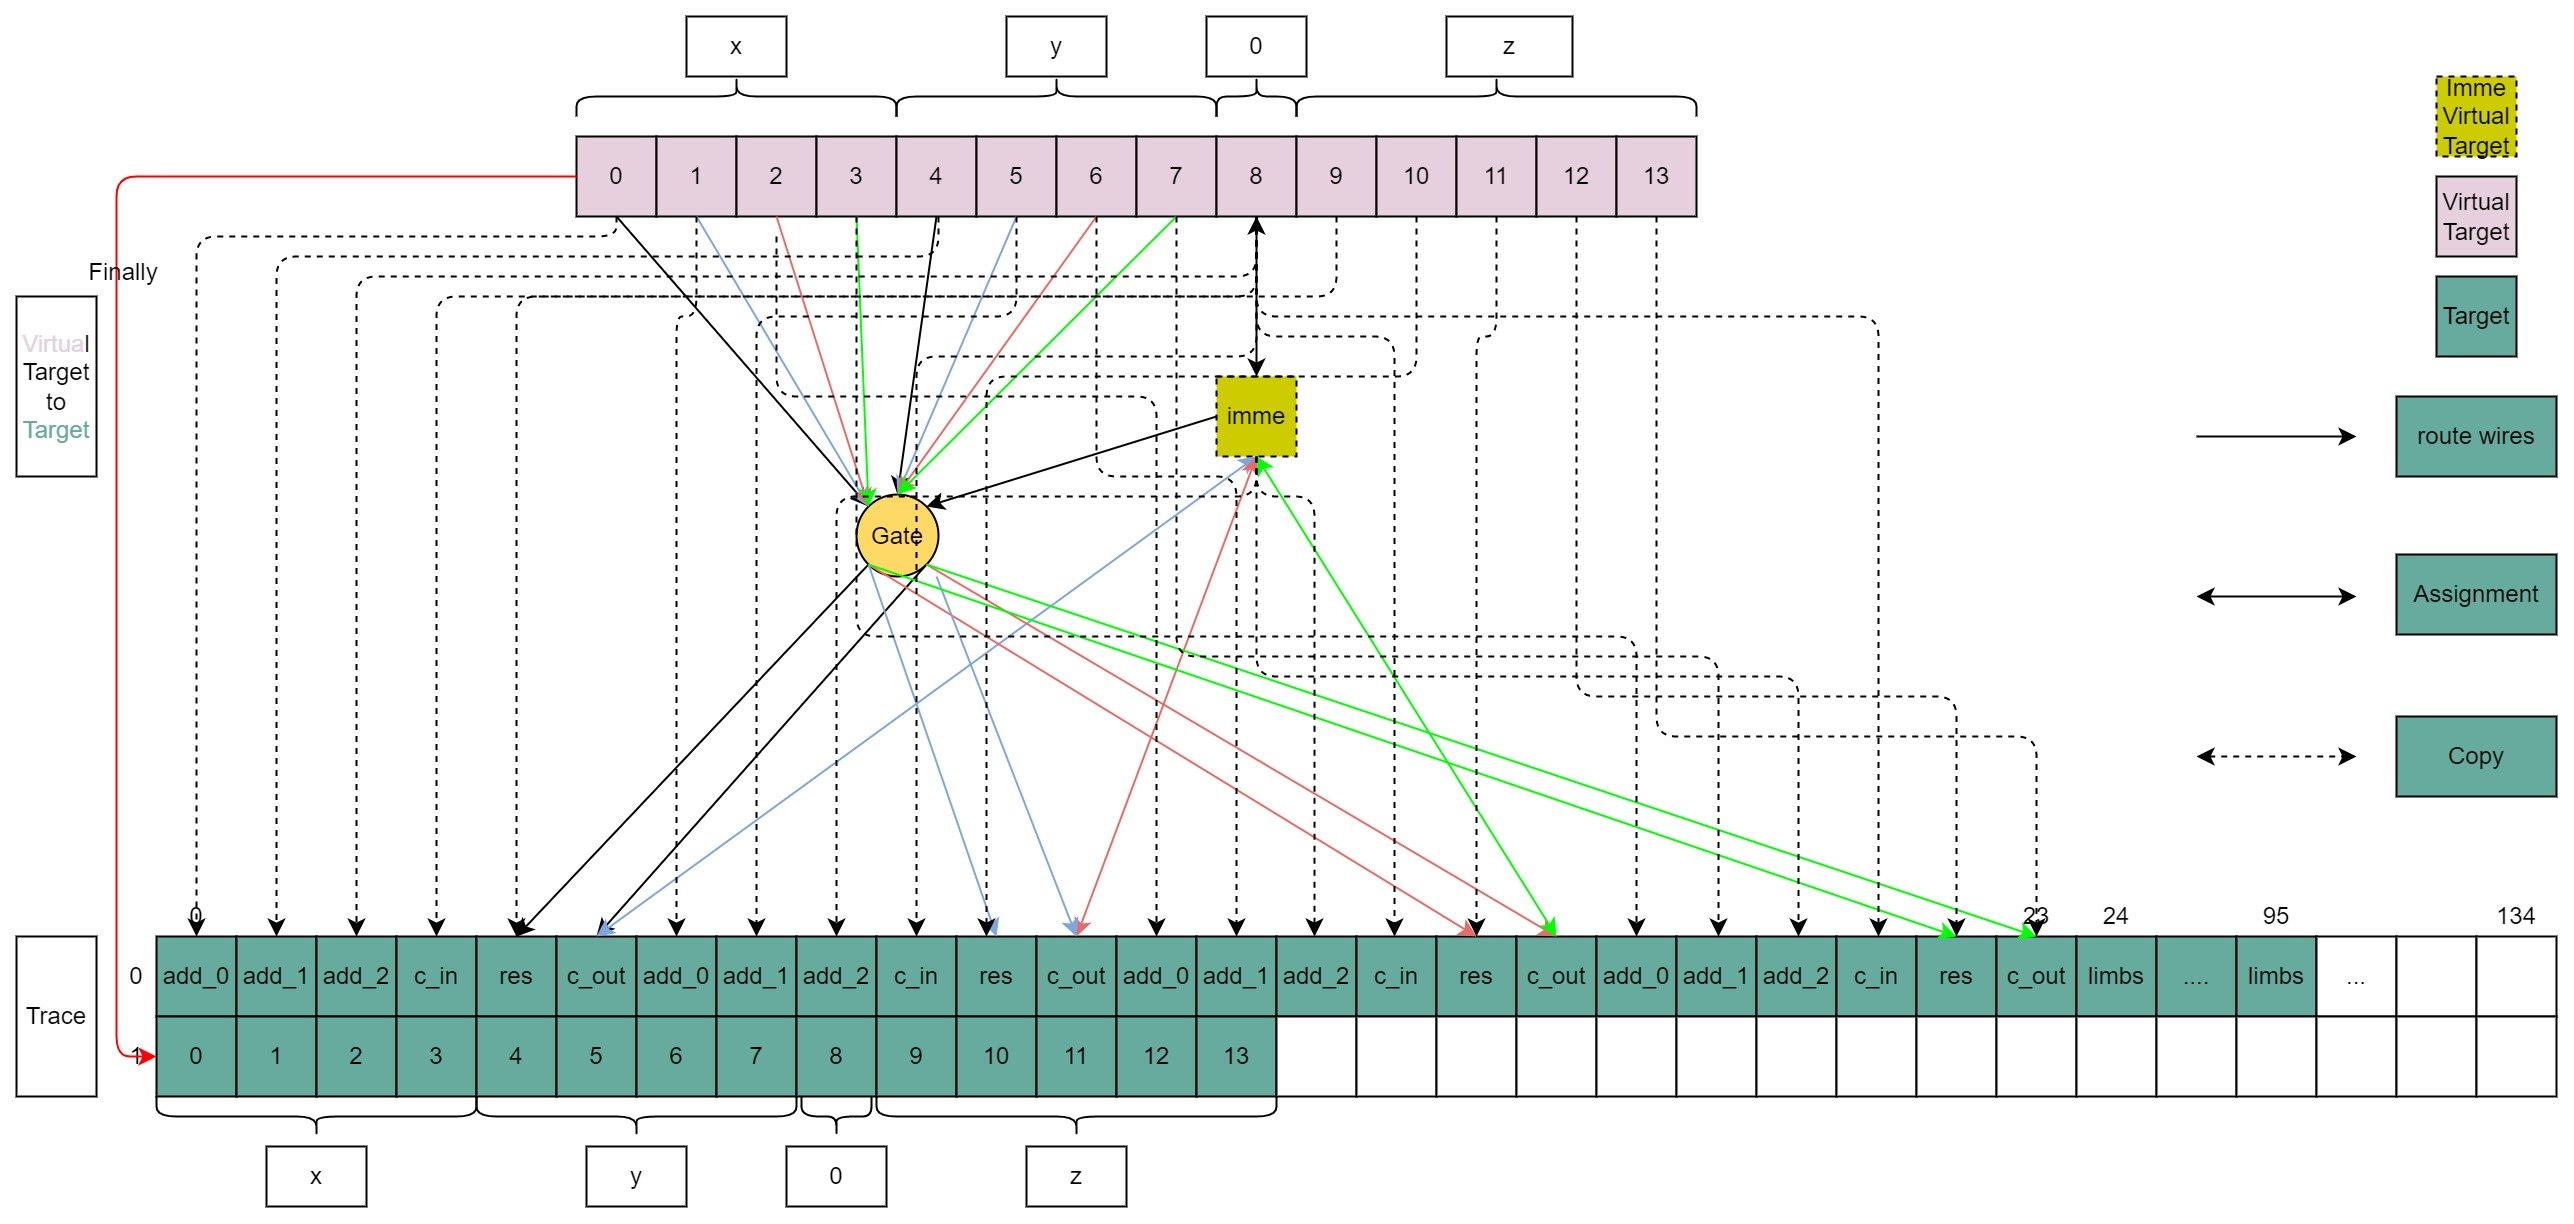
\includegraphics[width=0.8\textwidth]{add-biguint-trace-layout.jpg}
            \caption{Add-biguint trace layout}
            \label{fig:add-biguint-trace-layout}
        \end{figure}
    
    \item constraints-info and costs
        \begin{itemize}
            \item constraints-num: 5 * (3 + 32 / 2 + 4 / 2) = 105
            \item copy-constraints: 4 * 5 + 6 = 26
            \item max-degree: 4
            \item wires-num: 5 * (6 + 16 + 2) = 120
        \end{itemize}

    \item questions
        \begin{itemize}
            \item why not make rangecheck constraint for inputs?
            \item why not make copy constraint between cur-c-in and last-c-out?
        
        \end{itemize}

\end{enumerate}
    %\printbibliography[heading=bibintoc, title=\ebibname]%
\end{document}
